% !TeX program = xelatex
% Overleaf: Settings -> Compiler -> XeLaTeX.
\documentclass[11pt,a4paper,fontset=fandol]{ctexart}
\usepackage[margin=2.3cm]{geometry}
\usepackage{amsmath,amssymb}
\usepackage{enumitem}
\usepackage{tikz}
\usepackage{hyperref}
\hypersetup{colorlinks=true,linkcolor=blue,urlcolor=blue}
\setlength{\parindent}{0pt}
\setlength{\parskip}{0.5em}
\setlist[enumerate]{itemsep=0.25em,topsep=0.3em}
\setcounter{secnumdepth}{0}
\begin{document}
\section{GRE Mathematics 错题与不确定题：Practice 2}
本次收录 18、26、36、47、48、58、60、65、66，共 9 题。18、26 为名词理解不稳，47 为忘记方法后蒙对，48 为凭感觉答对；58 为审题，60、66 为抽象代数知识遗忘，65 为题意理解错误。36 按圈题收录，不额外推测具体错因。以下先保留原英文题干与选项，再解释关键词、推导答案并补充相关知识。

\subsection{18. Onto、矩阵空间的维数与核：A}
\label{p2:q18}
\textbf{原题（Original problem）}

Let $V$ be the real vector space of all real $2\times3$ matrices, and let $W$ be the real vector space of all real $4\times1$ column vectors. If $T$ is a linear transformation from $V$ onto $W$, what is the dimension of the subspace $\{\mathbf v\in V:T(\mathbf v)=\mathbf0\}$?

(A) $2$ \quad (B) $3$ \quad (C) $4$ \quad (D) $5$ \quad (E) $6$.

\textbf{名词解释。}real vector space：实向量空间；column vector：列向量；onto：满射（every element of the target is attained）；subspace：子空间；kernel/null space：核，即所有被映到零的输入；dimension：维数，即一组基中向量的个数。

\textbf{第一步：分清矩阵的尺寸与矩阵空间的维数。}$V$ 的一个元素是一整个 $2\times3$ 矩阵，而不是一列二维向量。这样的矩阵有 6 个可独立选择的实数位置，因此 $\dim V=6$。更具体地，令 $E_{ij}$ 表示只有第 $(i,j)$ 个位置为 1、其余位置全为 0 的矩阵，则
\[
A=\sum_{i=1}^{2}\sum_{j=1}^{3}a_{ij}E_{ij}.
\]
这 6 个矩阵线性无关且张成 $V$，故构成一组基。同理，$W=\mathbb R^4$，所以 $\dim W=4$。

\textbf{第二步：理解 onto。}题设说从 $V$ \emph{onto} $W$，不只是把输出放在 $W$ 里，而是 $W$ 中的每个向量都能被取到。因此 $\operatorname{im}T=W$，$\operatorname{rank}T=4$。

\textbf{第三步：识别所求子空间。}$\{\mathbf v\in V:T(\mathbf v)=\mathbf0\}=\ker T$。由秩--零度定理，
\begin{equation}
\dim V=\dim\ker T+\dim\operatorname{im}T,
\qquad \dim\ker T=6-4=\boxed{2}.
\label{p2:rank-nullity}
\end{equation}
因此选择 A；B--E 均不等于题设唯一确定的核维数。

\textbf{举一反三。}一般地，$m\times n$ 实矩阵的全体所构成的空间维数为 $mn$；一个具体矩阵的秩则至多为 $\min(m,n)$，两者是不同概念。对有限维线性映射，one-to-one/injective（单射）等价于 $\ker T=\{0\}$；onto/surjective（满射）等价于像空间等于目标空间。若本题只说 $T:V\to W$，没有 onto，就不能确定核维数恰为 2，只能知道它至少为 2。

\subsection{26. Relative extrema 与 absolute minimum：A}
\label{p2:q26}
\textbf{原题（Original problem）}

Let $f(x,y)=x^2-2xy+y^3$ for all real $x$ and $y$. Which of the following is true?
\begin{enumerate}[label=(\Alph*)]
\item $f$ has all of its relative extrema on the line $x=y$.
\item $f$ has all of its relative extrema on the parabola $x=y^2$.
\item $f$ has a relative minimum at $(0,0)$.
\item $f$ has an absolute minimum at $\left(\frac23,\frac23\right)$.
\item $f$ has an absolute minimum at $(1,1)$.
\end{enumerate}
\textbf{名词解释。}relative/local extremum：局部极值，extrema 是 extremum 的复数；relative minimum：局部极小值；absolute/global minimum：全局最小值；parabola：抛物线。题目中的 ``all of its relative extrema on the line'' 是说所有局部极值点都位于这条直线上，并非说直线上每个点都是极值点。

\textbf{定义。}$p$ 是局部极小值点，指存在 $\delta>0$，使得当 $\|q-p\|<\delta$ 时总有 $f(q)\ge f(p)$；只比较附近的点。全局最小值点要求对定义域中\emph{所有} $q$ 都有 $f(q)\ge f(p)$。局部极大值定义类似。鞍点（saddle point）附近同时有比它高和比它低的函数值，不是局部极值。

\textbf{求驻点。}由于定义域是整个 $\mathbb R^2$ 且 $f$ 可微，所有局部极值点都必须满足
\[
f_x=2x-2y=0,\qquad f_y=-2x+3y^2=0.
\]
第一式给 $x=y$，代入第二式得 $y(3y-2)=0$。因此只有两个驻点：$(0,0)$ 和 $(\frac23,\frac23)$。这一步已经说明所有局部极值点一定在 $x=y$ 上，故 A 正确。

\textbf{判别驻点并逐项排除。}Hessian 矩阵及其行列式为
\[
H_f(x,y)=\begin{pmatrix}2&-2\\-2&6y\end{pmatrix},\qquad D=12y-4.
\]
在 $(0,0)$，$D=-4<0$，是鞍点，C 错。也可不用 Hessian：沿 $y=0$ 有 $f(t,0)=t^2>0$，沿 $x=y=t$ 有 $f(t,t)=t^3-t^2<0$（$0<|t|<1$），而 $f(0,0)=0$。

在 $(\frac23,\frac23)$，$D=4>0$ 且 $f_{xx}=2>0$，所以它是严格局部极小值点。然而 $\frac23\ne(\frac23)^2$，它不在 $x=y^2$ 上，B 错。沿 $x=0,y\to-\infty$，$f(0,y)=y^3\to-\infty$，所以 $f$ 根本没有全局最小值，D、E 都错。

\textbf{相关方法。}二元 $C^2$ 函数在驻点处，若 $D=f_{xx}f_{yy}-f_{xy}^2>0$ 且 $f_{xx}>0$，则为局部极小值；$D>0,f_{xx}<0$ 则为局部极大值；$D<0$ 为鞍点；$D=0$ 时该判别法不能下结论。求全局最值时还必须检查边界及无穷远处，不能只求驻点。

\subsection{36. 两两线性无关不等于整体线性无关：A}
\label{p2:q36}
\textbf{原题（Original problem）}

Let $M$ be a $5\times5$ real matrix. Exactly four of the following five conditions on $M$ are equivalent to each other. Which of the five conditions is equivalent to NONE of the other four?
\begin{enumerate}[label=(\Alph*)]
\item For any two distinct column vectors $\mathbf u$ and $\mathbf v$ of $M$, the set $\{\mathbf u,\mathbf v\}$ is linearly independent.
\item The homogeneous system $M\mathbf x=\mathbf0$ has only the trivial solution.
\item The system of equations $M\mathbf x=\mathbf b$ has a unique solution for each real $5\times1$ column vector $\mathbf b$.
\item The determinant of $M$ is nonzero.
\item There exists a $5\times5$ real matrix $N$ such that $NM$ is the $5\times5$ identity matrix.
\end{enumerate}
\textbf{名词解释。}equivalent：等价，两个条件互相推出；distinct：不同的；homogeneous system：齐次方程组；trivial solution：零解；identity matrix：单位矩阵；linearly independent：线性无关。

\textbf{先核对 B--E。}对方阵，以下条件等价：可逆、满秩、行列式非零、齐次方程只有零解、每个右端向量对应唯一解。因此 B、C、D 等价。E 也等价：若 $NM=I$，取行列式得 $\det N\det M=1$，所以 $\det M\ne0$；反之若 $M$ 可逆，取 $N=M^{-1}$ 即可。

\textbf{A 只检查每次取两个列向量。}可逆当然保证所有列向量整体线性无关，因而任意两个列向量也线性无关；但反向不成立。考虑
\[
M=\begin{pmatrix}
1&1&1&1&1\\
0&1&2&3&4\\
0&0&0&0&0\\
0&0&0&0&0\\
0&0&0&0&0
\end{pmatrix}.
\]
第 $k$ 列形如 $(1,k-1,0,0,0)^T$。任意两列若互为倍数，由第一坐标可知倍数只能是 1，再由第二坐标可知它们应为同一列，矛盾。所以任意两列线性无关，满足 A。但整个矩阵秩为 2，行列式为零，不满足 B--E。因此 A 与其余四项均不等价，选 A。

\textbf{基本例子。}在 $\mathbb R^2$ 中，$(1,0),(0,1),(1,1)$ 两两线性无关，却满足第三个向量等于前两个之和。pairwise independent（两两无关）弱于整个向量组线性无关。

\subsection{47. 恒力做功与位移：C（答对但忘记方法）}
\label{p2:q47}
\textbf{原题（Original problem）}

Let $\mathbf F$ be a constant unit force that is parallel to the vector $(-1,0,1)$ in $xyz$-space. What is the work done by $\mathbf F$ on a particle that moves along the path given by $(t,t^2,t^3)$ between time $t=0$ and time $t=1$?

(A) $-\frac14$ \quad (B) $-\frac{1}{4\sqrt2}$ \quad (C) $0$ \quad (D) $\sqrt2$ \quad (E) $3\sqrt2$.

\textbf{名词解释。}constant force：恒力，即向量不随位置或时间变化；unit force：大小为 1 的力；parallel：平行；work：功；displacement：位移（终点减起点的向量）；distance traveled / arc length：路程（路径长度）。这里不是把力当作单位长度为 1 的路径。

\textbf{从定义计算。}令 $\mathbf r(t)=(t,t^2,t^3)$，则 $\mathbf r'(t)=(1,2t,3t^2)$。取 $\mathbf F=(-1,0,1)/\sqrt2$，则
\begin{equation}
W=\int_0^1\mathbf F\cdot\mathbf r'(t)\,dt
=\frac1{\sqrt2}\int_0^1(-1+3t^2)\,dt
=\frac1{\sqrt2}[-t+t^3]_0^1=\boxed0.
\label{p2:work-integral}
\end{equation}
平行也允许反方向；若取 $-\mathbf F$，上述功仍为 0，因此不影响答案。只有 C 正确。

\textbf{更快的方法。}恒力可以提到积分号外，故
\begin{equation}
W=\mathbf F\cdot\int_a^b\mathbf r'(t)\,dt
=\mathbf F\cdot\bigl(\mathbf r(b)-\mathbf r(a)\bigr).
\label{p2:constant-force}
\end{equation}
本题位移为 $(1,1,1)$，而 $(-1,0,1)\cdot(1,1,1)=0$。位移与力垂直，因此净功为零。

\textbf{纠正直觉。}应说“恒力的总功只与位移有关，与具体路径无关”，而不是“路程与位移无关”。路程是 $\int_a^b\|\mathbf r'(t)\|\,dt$，位移是 $\mathbf r(b)-\mathbf r(a)$，一般有路程 $\ge$ 位移的模。非零路程也可对应零功。只有力始终沿运动切线且大小恒定时，才能直接用“力的大小乘路程”。一般位置相关的力必须做线积分；保守场 $\mathbf F=\nabla\phi$ 的功为 $\phi(B)-\phi(A)$，同样与路径无关。

\subsection{48. 逐步核对中值定理论证：A（凭感觉答对）}
\label{p2:q48}
\textbf{原题（Original problem）}

Consider the theorem: If $f$ and $f'$ are both strictly increasing real-valued functions on the interval $(0,\infty)$, then $\lim_{x\to\infty}f(x)=\infty$. The following argument is suggested as a proof of this theorem.
\begin{enumerate}[label=(\arabic*)]
\item By the Mean Value Theorem, there is a $c_1$ in the interval $(1,2)$ such that
\[
f'(c_1)=\frac{f(2)-f(1)}{2-1}=f(2)-f(1)>0.
\]
\item For each $x>2$, there is a $c_x$ in $(2,x)$ such that $\frac{f(x)-f(2)}{x-2}=f'(c_x)$.
\item For each $x>2$, $\frac{f(x)-f(2)}{x-2}=f'(c_x)>f'(c_1)$ since $f'$ is strictly increasing.
\item For each $x>2$, $f(x)>f(2)+(x-2)f'(c_1)$.
\item $\lim_{x\to\infty}f(x)=\infty$.
\end{enumerate}
Which of the following statements is true?
\begin{enumerate}[label=(\Alph*)]
\item The argument is valid.
\item The argument is not valid since the hypotheses of the Mean Value Theorem are not satisfied in (1) and (2).
\item The argument is not valid since (3) is not valid.
\item The argument is not valid since (4) cannot be deduced from the previous steps.
\item The argument is not valid since (4) does not imply (5).
\end{enumerate}
\textbf{名词解释。}strictly increasing：严格递增，即 $x<y\Rightarrow f(x)<f(y)$；Mean Value Theorem：拉格朗日中值定理；hypotheses：定理的假设条件；valid argument：有效论证；deduce / imply：推导／推出。

\textbf{核对 (1)、(2)。}题目中 $f'$ 的存在意味着 $f$ 在 $(0,\infty)$ 可微，因而连续。因此在 $[1,2]$ 上连续、$(1,2)$ 内可微；在每个 $[2,x]$ 上同样满足条件。两次使用中值定理均合法，不要求 $f'$ 连续。由于 $f$ 严格递增，$f(2)>f(1)$，故得到固定常数 $m=f'(c_1)>0$。B 错。

\textbf{核对 (3)。}有 $c_1\in(1,2)$、$c_x\in(2,x)$，所以 $c_x>c_1$。这里用到的是\emph{导数函数} $f'$ 严格递增，故 $f'(c_x)>f'(c_1)=m$。C 错。区分“$f$ 递增”和“$f'$ 递增”：前者说函数值随自变量增大，后者说斜率随自变量增大。

\textbf{核对 (4)。}因为 $x-2>0$，把 (3) 乘以 $x-2$ 不改变不等号方向，移项即得 (4)。D 错。

\textbf{核对 (5)。}固定的 $m>0$ 使 $f(x)>f(2)+m(x-2)$，右端随 $x\to\infty$ 趋向 $\infty$，所以 $f(x)\to\infty$。若用定义说明，任给实数 $M$，只要 $x>\max\{2,2+(M-f(2))/m\}$，就有 $f(x)>M$。E 错，A 正确。

\textbf{可迁移的结论。}仅有 $f$ 严格递增不够，例如 $f(x)=1-e^{-x}$ 在 $(0,\infty)$ 递增却趋向 1。这里第二个条件保证从某一点之后斜率始终大于一个固定正数，从而函数至少以正斜率直线的速度增长。不要把“每一点的导数都为正”误当作“导数有统一正下界”；后者才直接保证这种线性增长。

\subsection{58. 相似矩阵的平移、迹与逆：E}
\label{p2:q58}
\textbf{原题（Original problem）}

Suppose $A$ and $B$ are $n\times n$ invertible matrices, where $n>1$, and $I$ is the $n\times n$ identity matrix. If $A$ and $B$ are similar matrices, which of the following statements must be true?
\begin{enumerate}[label=\Roman*.]
\item $A-2I$ and $B-2I$ are similar matrices.
\item $A$ and $B$ have the same trace.
\item $A^{-1}$ and $B^{-1}$ are similar matrices.
\end{enumerate}
(A) I only \quad (B) II only \quad (C) III only \quad (D) I and III only \quad (E) I, II, and III.

\textbf{名词解释。}similar matrices：相似矩阵，即存在\emph{可逆}矩阵 $S$ 使 $B=S^{-1}AS$；trace：迹，$\operatorname{tr}A=\sum_i a_{ii}$；inverse：逆矩阵。similar 与 symmetric（对称）不是同一概念。

\textbf{错因。}本题自述为审题；原卷中漏判了 II。先把 trace 译成“对角线元素之和”，再从相似关系直接计算。

I 正确，因为
\[
B-2I=S^{-1}AS-2S^{-1}IS=S^{-1}(A-2I)S.
\]
II 正确。利用 $\operatorname{tr}(XY)=\operatorname{tr}(YX)$，
\[
\operatorname{tr}B=\operatorname{tr}\bigl((S^{-1}A)S\bigr)
=\operatorname{tr}(SS^{-1}A)=\operatorname{tr}A.
\]
其中迹的循环性质可由 $\operatorname{tr}(XY)=\sum_{i,j}x_{ij}y_{ji}=\operatorname{tr}(YX)$ 直接证明。

III 正确。乘积取逆时顺序反转，故
\[
B^{-1}=(S^{-1}AS)^{-1}=S^{-1}A^{-1}S.
\]
所以三项全部成立，选 E；A--D 均漏掉至少一项。

\textbf{相关结论。}相似相当于同一个线性变换换一组基表示，因此保持特征多项式、特征值及代数重数、行列式、迹、秩和最小多项式。对任意多项式 $p$，$p(B)=S^{-1}p(A)S$；矩阵可逆时也能处理负整数幂。反过来，仅有相同迹、行列式或特征值不保证相似，例如 $I_2$ 与 $\begin{pmatrix}1&1\\0&1\end{pmatrix}$ 的这些量都相同，却不相似。

\subsection{60. 正五角星的对称群：E}
\label{p2:q60}
\textbf{原题（Original problem）}
\begin{center}
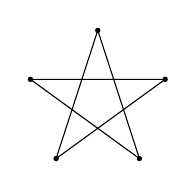
\begin{tikzpicture}[scale=0.75]
\foreach \k in {0,...,4}{\coordinate (v\k) at ({90+72*\k}:1.2);}
\draw (v0)--(v2)--(v4)--(v1)--(v3)--cycle;
\foreach \k in {0,...,4}{\fill (v\k) circle (1.3pt);}
\end{tikzpicture}
\end{center}
The group of symmetries of the regular pentagram shown above is isomorphic to the
\begin{enumerate}[label=(\Alph*)]
\item symmetric group $S_5$
\item alternating group $A_5$
\item cyclic group of order $5$
\item cyclic group of order $10$
\item dihedral group of order $10$
\end{enumerate}
\textbf{名词解释。}regular pentagram：正五角星；symmetry：保持图形的对称变换；group of symmetries：以变换复合为运算的对称群；isomorphic：同构；order of a group：群中元素个数；dihedral group：二面体群。这里的 symmetric group $S_5$ 是“对称群／置换群”的专有名词，不是说任何图形的对称群都等于 $S_5$。

\textbf{先回顾群的定义。}集合 $G$ 配备一个运算，若运算封闭、满足结合律、存在单位元且每个元素都有逆元，则称为群。图形对称变换的复合仍保持图形，什么都不做是单位元，每个旋转或反射都可以逆转，所以这些变换构成群。群同构是一个双射 $\varphi:G\to H$，还要求 $\varphi(ab)=\varphi(a)\varphi(b)$；不仅数目相同，运算结构也要相同。

\textbf{先数旋转。}绕中心旋转 $0^\circ,72^\circ,144^\circ,216^\circ,288^\circ$ 都保持五角星，共 5 个。令 $r$ 表示旋转 $72^\circ$，这 5 个变换是 $e,r,r^2,r^3,r^4$，且 $r^5=e$。

\textbf{再数反射。}有 5 条反射对称轴，每条经过一个外顶点和中心。令 $s$ 为其中一次反射，则其余反射可写为 $rs,r^2s,r^3s,r^4s$。所有平面对称共 10 个：5 个旋转和 5 个反射。这里计入整个图形的平面等距变换，不是对五个顶点任意重新编号。

\textbf{为什么是二面体群？}它与正五边形的对称群相同，满足
\[
r^5=e,\qquad s^2=e,\qquad srs=r^{-1}.
\]
最后一个关系表示“反射会把旋转方向反过来”。这是阶为 10 的二面体群，选 E。不同教材可能记作 $D_5$ 或 $D_{10}$，应以“阶为 10”识别，避免记号混淆。

\textbf{逐项排除。}A：$|S_5|=5!=120$，它允许任意置换，太多。B：$|A_5|=5!/2=60$，它只含偶置换，数量仍不对。C：阶 5 的循环群只描述旋转，漏了反射。D：阶 10 的循环群必须有一个阶 10 的生成元，但此处非恒等旋转的阶都是 5，反射的阶都是 2，没有阶 10 的元素；而且此群不交换，循环群必交换。因此不能只凭“有 10 个元素”选择 D。

\textbf{举一反三。}正 $n$ 边形的平面对称群有 $2n$ 个元素，包含 $n$ 个旋转与 $n$ 个反射；只允许旋转时得到阶 $n$ 的循环群。注意区分群的阶 $|G|$ 与元素的阶 $\operatorname{ord}(g)$（最小正整数 $k$ 使 $g^k=e$）。

\subsection{65. 连续满射与连续双射：B}
\label{p2:q65}
\textbf{原题（Original problem）}

Which of the following statements are true about the open interval $(0,1)$ and the closed interval $[0,1]$?
\begin{enumerate}[label=\Roman*.]
\item There is a continuous function from $(0,1)$ onto $[0,1]$.
\item There is a continuous function from $[0,1]$ onto $(0,1)$.
\item There is a continuous one-to-one function from $(0,1)$ onto $[0,1]$.
\end{enumerate}
(A) None \quad (B) I only \quad (C) II only \quad (D) I and III only \quad (E) I, II, and III.

\textbf{审题重点。}from 指定义域，onto 指满射，要求\emph{值域恰好等于}后面的集合；one-to-one 指单射，即不同输入有不同输出。I 只要求连续满射，允许重复取值；III 同时要求连续、单射、满射，明显比 I 强。``There is'' 是存在至少一个函数，不是每个函数都满足。

\textbf{I 正确：直接构造。}令
\[
f:(0,1)\to[0,1],\qquad f(x)=\sin^2(2\pi x).
\]
它连续且值总在 $[0,1]$。在定义域内的点上，$f(\frac14)=1$、$f(\frac12)=0$。由介值定理，在 $[\frac14,\frac12]\subset(0,1)$ 上能取到 0 与 1 之间每个值，所以满射到 $[0,1]$。目标集合包含端点，并不要求定义域也包含端点；输出为 0 或 1 的输入可以是内部点。

\textbf{II 错误：连续函数在闭有界区间上达到最值。}若连续 $g:[0,1]\to(0,1)$ 为满射，则其值域应为 $(0,1)$。但极值定理保证存在 $a,b\in[0,1]$，使 $m=g(a)$ 是最小值、$M=g(b)$ 是最大值。由于所有函数值都在 $(0,1)$，有 $0<m\le M<1$。例如 $m/2\in(0,1)$ 不可能被取到，与满射矛盾。也可说紧集 $[0,1]$ 的连续像必须紧，而 $(0,1)$ 不紧。

\textbf{III 错误：单射造成障碍。}反设存在连续单射满射 $h:(0,1)\to[0,1]$。满射要求存在 $a\in(0,1)$ 使 $h(a)=0$。选 $u<a<v$，都在 $(0,1)$ 中。由于单射且函数值非负，$h(u)>0$、$h(v)>0$。取 $c=\frac12\min\{h(u),h(v)\}>0$。介值定理分别作用于 $[u,a]$ 和 $[a,v]$，得到 $u<\xi<a<\eta<v$ 且 $h(\xi)=h(\eta)=c$，与单射矛盾。因此不存在这样的 $h$。

相关结论是：实区间上的连续单射必严格单调；而开区间上的严格单调函数不可能在内部取得全局最小值 0 和最大值 1。只知道两个集合等势（存在集合意义的双射），不能推断存在连续双射。最终只有 I 正确，选 B。

\subsection{66. 只有两个右理想的含幺环：B}
\label{p2:q66}
\textbf{原题（Original problem）}

Let $R$ be a ring with a multiplicative identity. If $U$ is an additive subgroup of $R$ such that $ur\in U$ for all $u\in U$ and for all $r\in R$, then $U$ is said to be a right ideal of $R$. If $R$ has exactly two right ideals, which of the following must be true?
\begin{enumerate}[label=\Roman*.]
\item $R$ is commutative.
\item $R$ is a division ring (that is, all elements except the additive identity have multiplicative inverses).
\item $R$ is infinite.
\end{enumerate}
(A) I only \quad (B) II only \quad (C) III only \quad (D) I and II only \quad (E) I, II, and III.

\textbf{先回顾定义。}环的加法构成交换群，乘法满足结合律，且乘法对加法满足左右分配律。含幺环（ring with a multiplicative identity）另有元素 $1$ 满足 $1r=r1=r$。加法单位元是 $0$，不要与乘法单位元 $1$ 混淆。

加法子群 $U$ 满足 $0\in U$ 且 $u-v\in U$（$u,v\in U$）。右理想在此基础上还要求 $ur\in U$（$u\in U,r\in R$），即理想元素放左边，右乘任意环元素后仍在理想中。左理想要求 $ru\in U$；双侧理想两个方向都要求。除环（division ring）是 $1\ne0$ 且每个非零元素均有双侧乘法逆元的环，\emph{不要求}乘法交换；再要求乘法交换才是域（field）。

\textbf{第一步：恰好是哪两个右理想？}$\{0\}$ 和 $R$ 永远是右理想。若 $R$ 为零环，它们相同，只有一个右理想；本题恰有两个，故 $1\ne0$，且只有 $\{0\}$、$R$ 两个右理想。

\textbf{第二步：从任意非零元素构造右理想。}任取 $a\ne0$，考虑
\[
aR=\{ar:r\in R\}.
\]
它是右理想：$0=a0\in aR$；$ar_1-ar_2=a(r_1-r_2)\in aR$；$(ar)t=a(rt)\in aR$。又因为 $a=a1\in aR$ 且 $a\ne0$，所以它不是零理想，只能有 $aR=R$。因此 $1\in aR$，存在 $b\in R$ 使
\begin{equation}
ab=1.
\label{p2:right-inverse}
\end{equation}
这只先证明 $b$ 是 $a$ 的\emph{右逆}，不能未经证明就改写为 $ba=1$。

\textbf{第三步：把右逆变成双侧逆。}由 $ab=1$ 知 $b\ne0$，对 $b$ 重复第二步，得到某个 $c\in R$ 使 $bc=1$。由结合律，
\[
a=a(bc)=(ab)c=c.
\]
于是 $ba=bc=1$。结合 $ab=1$，得到 $b$ 是 $a$ 的双侧逆。由于 $a\ne0$ 任意，所有非零元素都可逆，II 正确。

\textbf{I 不一定成立。}实四元数环 $\mathbb H=\{a+bi+cj+dk:a,b,c,d\in\mathbb R\}$ 是非交换除环，其乘法满足 $i^2=j^2=k^2=-1$、$ij=k$、$ji=-k$。每个非零四元数 $q=a+bi+cj+dk$ 都有逆
\[
q^{-1}=\frac{a-bi-cj-dk}{a^2+b^2+c^2+d^2}.
\]
除环的非零右理想若含 $q\ne0$，由右吸收性含 $qq^{-1}=1$，继而含 $1r=r$（任意 $r\in R$），所以必为整个环。因此四元数环恰有两个右理想，却不交换，否定 I。GRE 中需要认识这个标准反例，不必在本题展开构造四元数乘法。

\textbf{III 不一定成立。}有限域 $\mathbb F_2=\mathbb Z/2\mathbb Z=\{0,1\}$ 有乘法单位元，唯一非零元素 1 可逆，故恰有两个右理想，却是有限集合。因此 III 错。只有 II 必然成立，选 B。

\textbf{举一反三。}含幺非零环中，只要某个右理想包含 1，它就等于整个环。交换含幺非零环只有两个理想，当且仅当它是域；不预设交换时，只有两个\emph{右}理想推出除环。不要把条件擅自弱化成“只有两个\emph{双侧}理想”：矩阵环 $M_n(\mathbb R)$（$n\ge2$）只有零理想与全环两个双侧理想，但包含非零不可逆矩阵，不是除环。左右条件在非交换环中确实重要。

\subsection{本套复习清单}
\begin{itemize}
\item 18、26：把 onto、relative、absolute 等词先译准，再套定理；矩阵空间维数与矩阵秩必须分开。
\item 36、58：区分两两无关与整体无关；相似矩阵保持迹，优先写出 $B=S^{-1}AS$。
\item 47：从功的线积分出发；恒力用力与位移的点积，不能用力的大小乘路程。
\item 48：逐步检查中值定理条件、不等号方向和固定正下界，不靠图形感觉判断论证。
\item 60、66：先记群、群的阶、循环群、二面体群，以及右理想、除环、域的定义；反例分别记正五边形对称群、四元数环和有限域。
\item 65：把 from、onto、one-to-one 分开读。连续满射可以重复取值；紧集的连续像是紧集。
\end{itemize}
\end{document}
